\documentclass{article}
\usepackage[margin=1in]{geometry} % For better margins
\usepackage{graphicx} % Required for \rotatebox command
\usepackage{booktabs} % For better table formatting
\usepackage{caption} % For table caption customization
\usepackage{enumitem}

\title{Exercise sheet Nr. 2}
\author{Ichim Stefan - ICA - 246/1}
\date{\today}

\begin{document}

\maketitle

\left(\textbf{G 1}\right) \textbf{Line}\ \textbf{diagram}

\begin{enumerate}[label=\alph*)]
  \item \textbf{Define:} What is a lattice? \\
      A lattice is a graphical representation which is used to represent hierarchical relationships between formal concepts.

  \item Find a preferably small lattice and draw its diagram. \\
  \begin{figure}[htbp]
    \centering
    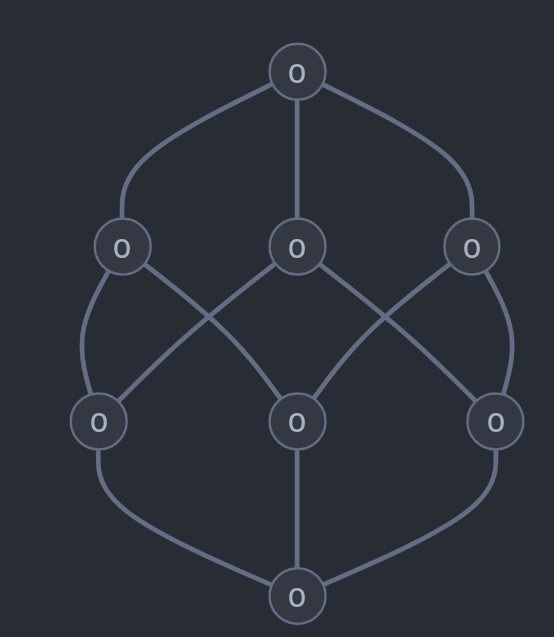
\includegraphics[width=0.4\textwidth]{g1b_lattice.png}
    \caption{Lattice}
    \label{fig}
  \end{figure}

\item Which of the following line diagrams (see Figure \ref{order_diagrams}) does not represent a lattice? Why? \\
  \begin{figure}[htbp]
    \centering
    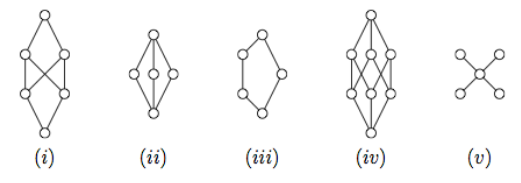
\includegraphics[width=0.5\textwidth]{g1c_lattices.png}
    \caption{Order diagrams}
    \label{order_diagrams}
  \end{figure}
    Diagram $(v)$ lacks the supremum and infimum which are crucial characteristics of concept lattices. There are no clear top and bottom elements, and the property that each pair of elements must have a unique supremum and unique infimum isn't met. This can be seen if we take any outer node in consideration.

\end{enumerate}

\left(\textbf{G 2}\right) \textbf{Complete}\ \textbf{lattice}

\begin{enumerate}[label=\alph*)]
  \item \textbf{Define:} What is a complete lattice? \\
    A complete lattice is a lattice where every subset of elements (elements at the same level in the hierarchy) has a supremum and infimum.

  \item Can you find a complete lattice among the lattices of Exercise 1c? \\
    Diagrams $(i)$ to $(iii)$ are complete lattices. We can find a supremum and infimum for each subset of nodes at the same level

  \item Can you give an example of a lattice which is not a complete lattice?\\
    Diagram $(iv)$ is an incomplete lattice. If we look at the second row from top to bottom, if we take the whole subset of nodes, there is no common infimum, and if we look at the third row from top to bottom, if we take the whole subset of nodes again, there is no common supremum.

\end{enumerate}

\left(\textbf{G 3}\right) \textbf{Formal}\ \textbf{Concepts}

Try to compute all formal concepts of the formal context shown in Figure \ref{grobian_gans}


  \begin{figure}[htbp]
    \centering
    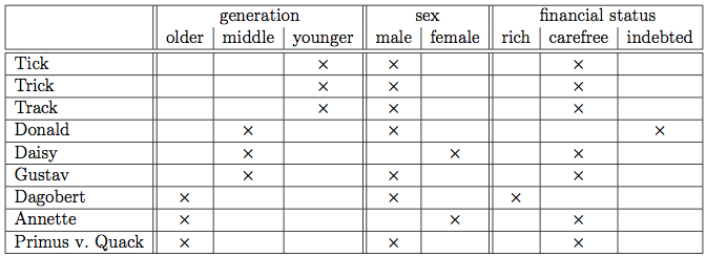
\includegraphics[width=0.9\textwidth]{g3_concepts.png}
    \caption{Grobian Gans: Die Ducks. Pshycogramm einer Sippe. Rowohlt, Reinbek bei Hamburg 1972, ISBN 3-499-11481-X}
    \label{grobian_gans}
  \end{figure}

\begin{itemize}
    \item $(\{\text{Tick, Trick, Track}\}, \{\text{younger, male, carefree}\})$
    \item $(\{\text{Donald}\}, \{\text{middle, male, indebted}\})$
    \item $(\{\text{Daisy}\}, \{\text{middle, female, carefree}\})$
    \item $(\{\text{Gustav}\}, \{\text{middle, male, rich}\})$
    \item $(\{\text{Dagobert}\}, \{\text{older, male, rich}\})$
    \item $(\{\text{Annette}\}, \{\text{older, female, carefree}\})$
    \item $(\{\text{Primus v. Quack}\}, \{\text{older, male, carefree}\})$
    \item $(\{\text{Tick, Trick, Track, Donald, Gustav, Dagobert, Primus v. Quack}\}, \{\text{male}\})$
    \item $(\{\text{Tick, Trick, Track, Daisy, Annette}\}, \{\text{carefree}\})$
    \item $(\{\text{Donald, Daisy, Gustav}\}, \{\text{middle}\})$
    \item $(\{\text{Dagobert, Annette, Primus v. Quack}\}, \{\text{older}\})$
    \item $(\{\text{Tick, Trick, Track}\}, \{\text{younger}\})$
    \item $(\{\text{Daisy, Annette}\}, \{\text{female}\})$
    \item $(\{\text{Dagobert}\}, \{\text{rich}\})$
    \item $(\{\text{Donald}\}, \{\text{indebted}\})$
    \item $(\{\text{Tick, Trick, Track, Primus v. Quack, Annette}\}, \{\text{carefree}\})$
    \item $(\{\},\{\text{older, middle, younger, male, female, rich, carefree, indebted}\})$
    \item $(\{\text{Tick, Trick, Track, Donald, Daisy, Gustav, Dagobert, Annette, Primus v. Quack}\}, \{\})$
\end{itemize}

\end{document}
